\team{I would merge this section with Introduction}

\subsection{Task Overhead}

\team{I think we should frame this "task overheads" into a bigger picture. Starting by explaining how the process of running a Spark streaming application works, and then pointing out the major sources of overhead. Plot graph showing the time breakdown between serialization, computation, scheduling, etc...}

Since tasks form the basic units of computation for Spark Streaming, it is important to optimize its execution. 
\jianneng{I don't agree with the previous statement. Tasks are also the basic units for computation in Hadoop and still that is not such a big deal because batch tasks take a lot of time. Next sentence is good and should be more developed.} 
This problem is especially relevant in our case, since the tasks we are executing are short. As the system is still relatively new, much of the current codebase emphasizes more on the ease of understanding over raw performance. 
\jianneng{Previous sentence sounds very software engineery. In systems papers we usually don't see this types of comments.}
By analyzing the decisions made by the developers and measuring execution times in different sections of the code path, we found a number of inefficiencies that can be improved upon.

For every Spark Streaming application, there is a driver and multiple executors. The receivers of data run on executors, and these receivers send to the driver metadata about the blocks generated. After every batch interval, the driver collects all of the blocks received during the period and make them into a RDD (Resilient Distributed Dataset, Spark's abstraction for distributed objects), and runs application logic on it using Spark. Spark runs each function on the RDD by generating tasks, serializing them, and sending them to appropriate executors. The executors deserialize each task, runs the function, and returns to the driver the results.

During our experiments, we found that when a task is not computation-intensive, the majority of the time in running the task is spent in deserialization. When running tasks with no-op operations, we found that from the driver's perspective, the time it takes for a task to be scheduled to the time it takes for the result to be received is 5ms. However, approximately 3.6ms out of this time is spent deserializing the task. These metrics mean that if we can reduce the task deserialization time, there will be a considerable improvement to the latency of small tasks.
\jianneng{We should show a more principled approach of getting to these results/conclusions. Here we should setup an experiment, explain how it was run, run it and show graphs with results. From this experiment and graphs come the conclusions. I tried to do this below in the "Scheduling scalability" benchmark}

\begin{figure}[t!]
  \begin{center}
    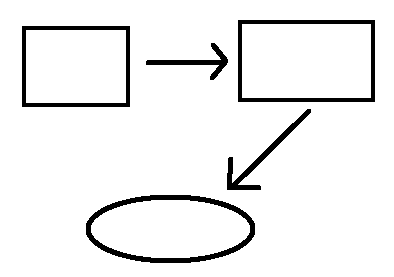
\includegraphics[scale=0.30]{images_graphs/spark_diagram.png}
  \end{center}
  \caption{Diagram of a Spark Streaming execution}
  \label{fig:deserialization}
\end{figure}

\begin{figure}[t!]
  \begin{center}
    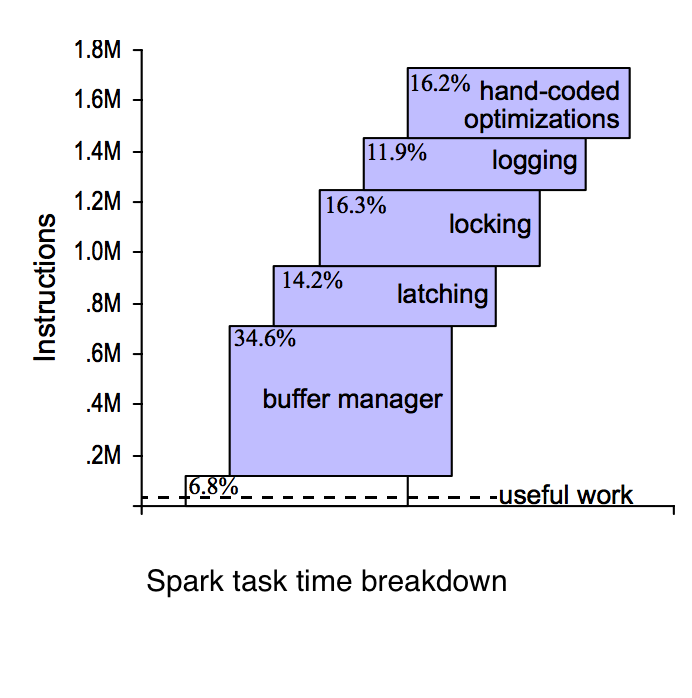
\includegraphics[scale=0.30]{images_graphs/time_breakdown.png}
  \end{center}
  \caption{Spark streaming task time breakdown (Dummy)}
  \label{fig:deserialization}
\end{figure}

\begin{figure}[t!]
  \begin{center}
    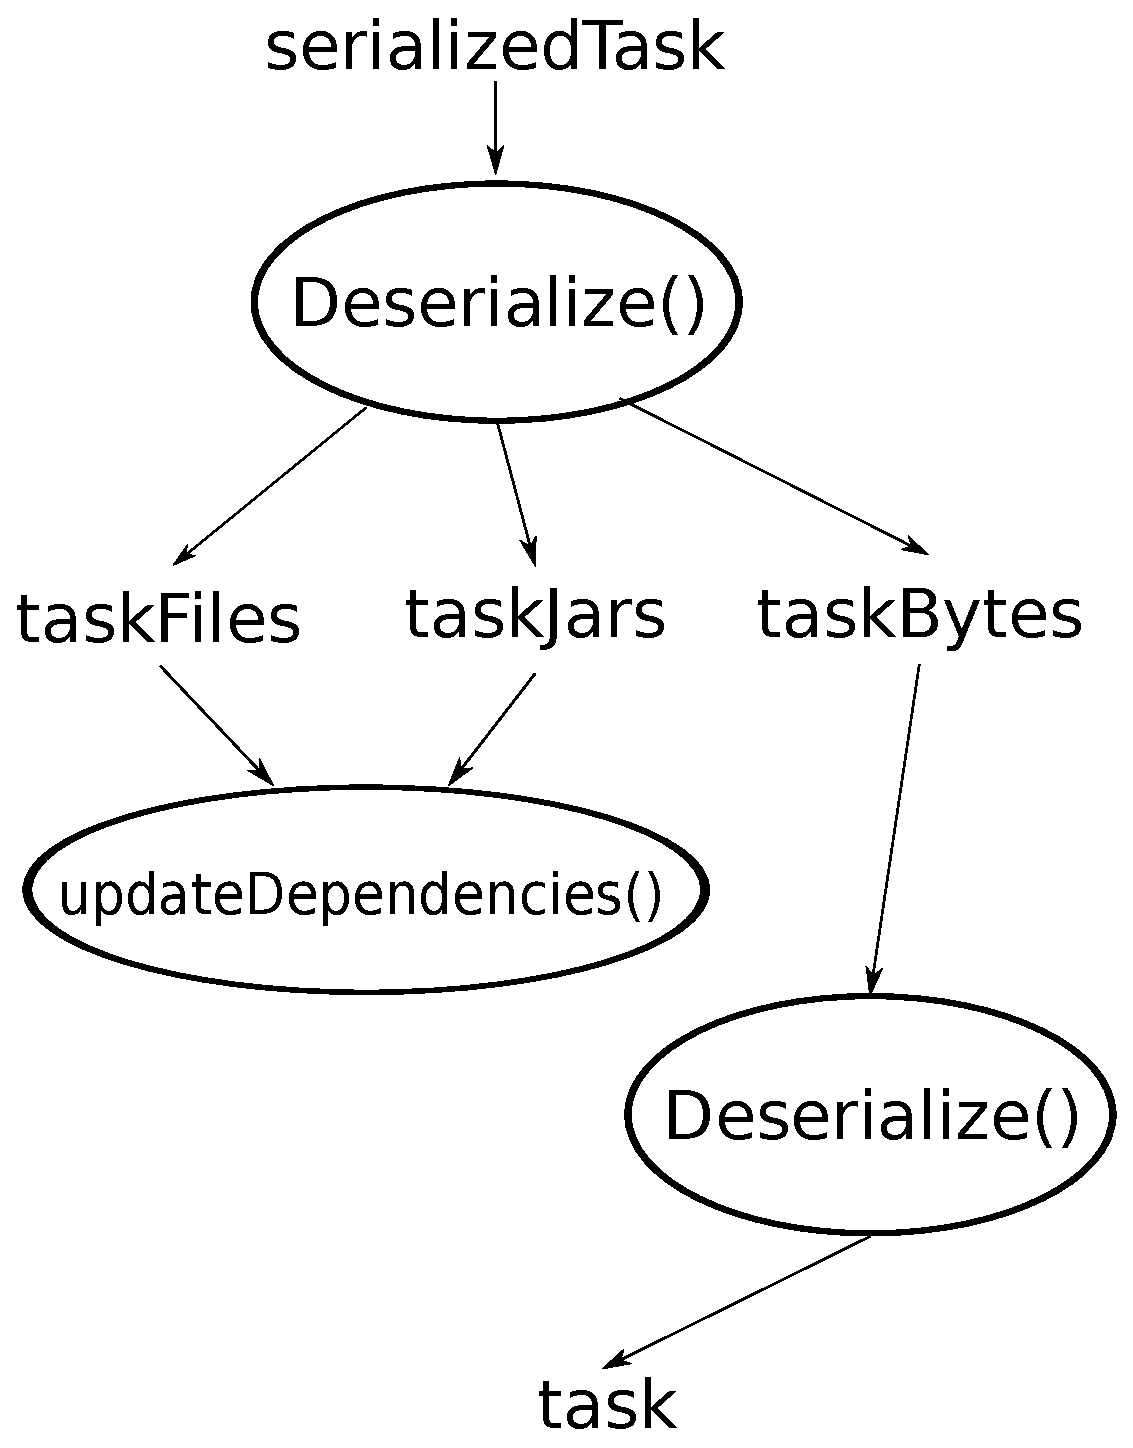
\includegraphics[scale=0.30]{images_graphs/deserialization.eps}
  \end{center}
  \caption{How a task is deserialized on the executor. \jianneng{expand this caption? The diagram is interesting and this description can be more developed. E.g., its not clear what the dependencies are}}
  \label{fig:deserialization}
\end{figure}

\subsection{Scheduling Scalability}

During the execution of a Spark Streaming application, the Driver (a central component of Spark) generates tasks periodically and adds them to the tail of a scheduling queue. This queue is continuously probed by the scheduler, which schedules by taking tasks from the queue and sending them to worker nodes for processing.
As applications specify lower batch intervals to process results more quickly, the number of tasks added to the queue per unit of time increases. Eventually, the scheduler will be unable to keep up with the rate of tasks being added to the queue. This results in an indefinite increase in the average time to schedule a task, which is worse considering the fact that tasks in one batch have less time to be processed before the next batch is generated.
From this observation, we can see that lower batch intervals lead to lower task latencies, less throughput and more tasks scheduled per second. On the other hand, larger batch intervals lead to higher throughput, higher task latencies and less tasks scheduled per second. 

To understand the performance of the current version of Spark Streaming, we have benchmarked the end-to-end latencies of tasks with different batch intervals. 
Our benchmarks were run on a 16-node cluster, with each node having 16 cores. We have used 120 receivers on 4 nodes. 
With this configuration, Spark Streaming generates 120$*$1000/(batch interval) tasks per second.
Because we are solely interested in benchmarking the scheduling performance, we ran applications that generate no-op tasks.

We have found that for a batch interval less than 40ms the system becomes unstable because the scheduler cannot keep up with the rate of tasks generated. This instability leads to increasingly higher scheduling delays and increasing garbage collection activity due to higher memory usage. \joao{Need a graph here showing end-to-end latency of tasks with varying batch intervals}


\subsection{Network Overhead}
As the number of tasks increases, so does the amount of communication between the driver and executors. We plan to increase the network throughput using InfiniBand, and also explore using RDMA to realize zero-copy. Ideally with these improvements, not only network communication will be faster, the driver will also have more CPU time to schedule tasks, ultimately reducing the latencies of running tasks.


\begin{figure}[t!]
  \begin{center}
    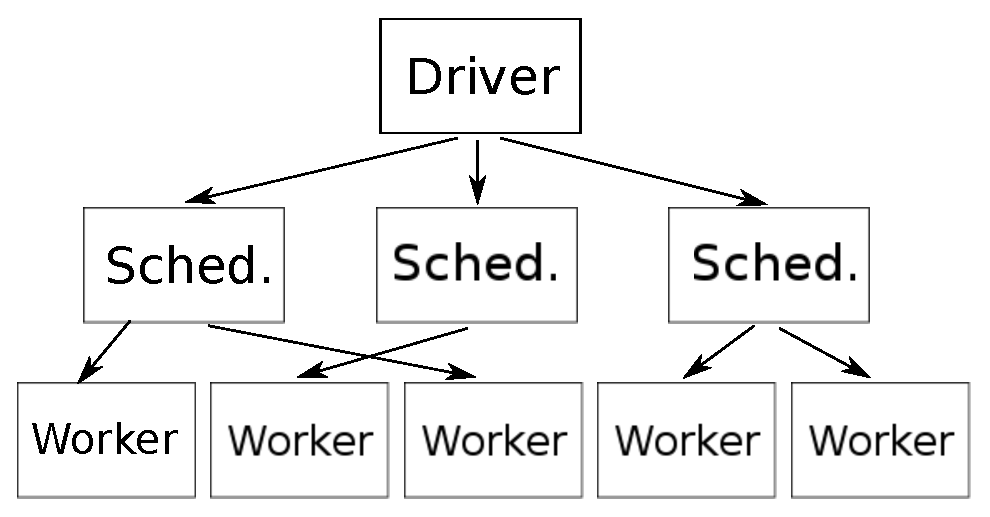
\includegraphics[scale=0.45]{images_graphs/scheduler_architecture.eps}
  \end{center}
  \caption{Proposed scheduler architecture. Schedulers are elastically spawned by the driver. These schedulers receive tasks from the Driver and schedule them to Worker nodes.}
  \label{fig:schedarch}
\end{figure}

